\section{Goal}
The goal of this project is to implement an image segmentation algorithm 
as described in \cite{felzen04}. In their work the authors give an overview of the possible 
approaches and related work and suggest a clear and easy to understand graph-based algorithm to solve the problem. 
The authors first describe the basic idea for segmenting the image, then propose various
ways to make it better. They claim that the method is fast and can run in fractions of a second for medium size input.

The algorithm and it's variations shall be implemented in python and compared in both speed and quality.


\section{Image Segmentation}
Image segmentation is the process of dividing the digital image into different components. The components are composed
of pixels that are somehow similar. In this work we shall be comparing pixels using their color intensities and later
also using the Euclidean distance between them. At the end of the process the image is divided into multiple components
with random colour assigned to each component making it distinct from its neighbours. Image segmentation
has many applications in areas like computer vision and image processing. A similar problem of edge detection in an
image can also be solved with segmentation.


\section{Building the Graph}
In \cite{felzen04} the authors view an image as a graph where each pixel is a vertex. They then describe two approaches to 
connect the vertices with edges. 

The first one is to connect every pixel with all 8 of it's neighbouring vertices.
In this case the graph of $n$ vertices has $4n$ edges because the edges are undirected. Similarly, only 4 neighbours can be
considered, this would reduce the number of edges to $2n$. 
The weight function between the vertices is defined as the Euclidian distance of intensities of each colour channel.
For example, if there are two pixels in RGB colour space $a = (r1,g1,b1)$ and $b = (r2,g2,b2)$ then their distance is:
\[
w_1(a,b) = \sqrt{(r1-r2)^2 + (g1-g2)^2 + (b1-b2)^2}
\]

The second approach is to consider the neighbouring vertices within a certain radius and only choose $l$ lowest weight edges.
In this case the graph would have $ln$ edges. Here the weight function depends both on the colour intensities and the distance
between the pixels. Assuming that $a$ has coordinates $(x1,y1)$ and b has coordinates $(x2,y2)$:
\[
w_2(a,b) = \sqrt{(x1-x2)^2 + (y1-y2)^2 + (r1-r2)^2 + (g1-g2)^2 + (b1-b2)^2}
\]

As shall be seen from the algorithm, both the speed and the quality of the segmentation depend on the number of edges in
the graph, therefore it is important to find a suitable balance.

\section{The Algorithm}
The input is a graph $G = (V, E)$ with $n$ vertices and $m$ edges. The output is a segmentation of $V$ into a set of components 
$S = (C_1,...,C_r)$.

We define internal difference for component $C$ to be the the edge with the largest weight in the MST (minimum spanning tree) of this 
component. That is:
\[
Int(C) = max\ w(e), e \in MST(C,E)
\]

We also define a threshold function to be:
\[
\tau = K / |C|
\]
where $K$ is a constant and $|C|$ is the number of pixels in component $C$. The choice of $K$ depends on the input,
if $K$ is big, the size of the components in the final segmentation tends to also be big.

The algorithm is as follows:
\begin{enumerate}
\item Sort the edges by non-decreasing edge weight.
\item Start with a segmentation $S^0$ where each vertex is in its own separate component.
\item For each edge $e_q$, where $q = 1..m$, construct $S^q$ using $S^{q-1}$. Let $e_q = (u, v)$. 
If $u$ and $v$ are in the same component in $S^{q-1}$ then we do nothing and continue with the next edge.
Otherwise, let $C_u$ be the component containing $u$ and $C_v$ be the component containing $v$, then if
\[
w(e_q) \leq min(Int(C_u) + \tau(C_u), Int(C_v) + \tau(C_v)) 
\]
we merge $C_u$ and $C_v$ and obtain $S^q$.
\item output $S^m$
\end{enumerate}

This algorithm is very similar to Kruskal's algorithm for finding a minimum spanning tree. Description and analysis of the algorithm
can be found in \cite{cormen01}. We implement the segmentation data structure, $S$, as a disjoint set with path compression and union by rank heuristics.
Disjoint sets are also described in \cite{cormen01}. 

The sorting of edges in step 1 takes $\Theta(m\log m)$ time. Since after each merge operation in 
step 3 we can remember the new largest weight edge $e_q$, the $Int(C)$ operation takes constant time. Merge operation for a disjoint set with
path compression and union by rank heuristics is an extremely slowly-growing function, it can be considered a constant in practice. In total
step 3 takes $\Theta(m)$ time and thus the whole algorithm is $\Theta(m\log m)$.

\section{Quality Improvement Methods}
There is a number of techniques to improve the segmentation quality. 

The first one is to use a Gaussian blur (\cite{wiki01}) filter before running the algorithm to reduce image noise and hopefully allow more components 
to merge together. The filter takes $\sigma$ as a parameter, when it is small the filter does not change the image significantly. 
$\sigma$ is a constant and can be set manually.

The other technique is the post-processing of components. When the algorithm finishes, we look at every edge again and if its vertices
belong to different components and one of these components has a size smaller than some $Min_c$ then we merge the components together.
This makes sure that every component has at least $Min_c$ pixels. $Min_c$ is a constant and can be set manually.

\section{Implementations in Python}
Three implementations were made in python. All of them are using the same segmentation algorithm, but handle input or build the graph differently.
All three use Gaussian blur and component post-processing.

The first implementation builds an 8-connected graph and runs the algorithm once. The edge weight function is $w_1$ as defined in Section 3.

The second implementation splits the input image into 3 colour channels (assuming it is RGB), builds 3 graphs and runs the algorithm once for
each graph. It then combines three disjoint sets into one by placing two vertices connected by an edge into the same component only if they are
in the same component in all three disjoint sets. 
The edge weight function is simply the absolute difference of the pixel intensities for the given colour channel.

The third implementation builds the graph according to the second approach from Section 3 by looking within a certain radius $R$ around each 
vertex and choosing $l$ best neighbours. The algorithm is then run once on the resulting graph. The radius $R$ and $l$ are constants and can 
be set manually.
This implementation produces segmentation of the best quality.

\section{Comparison}
The comparison of the three implementations is given in table~\ref{table1}. The input and output images are presented in Appendix A, figure~\ref{fig:car200}.

Overall all three python implementations turned out to be very slow, taking time from several seconds to several minutes for different input.
The slowness is due partly to python itself and partly to the representation of the image in memory as an object rather than a simple array
of values. Implementations in languages such as C or C++ are expected to be significantly faster.



\begin{table}[h]
    \begin{tabular}{| l | l | l | l |}
    \hline
Implementation              &   First     & Second       & Third ($R = 15, l = 8$) \\ \hline
Graph construction time     &   2.525915  & 3 x 1.45     & 24.584158 \\
Segmentation time           &   4.073868  & 3 x 3.93     & 6.265604 \\
Post-processing (PP) time   &   3.497167  & 3.490101     & 7.009409 \\
Edges                       &   105403    & 3 x 105403   & 212788 \\
Components before PP        &   216       & 1844         & 223 \\
Components after PP         &   69        & 212          & 33 \\ \hline
Time total                  &   10.731729 & 28.876814    & 38.679581 \\ 
    \hline
    \end{tabular}

    \caption{Comparison for a 200x133 pixel RGB image in figure~\ref{fig:car200}. All time values are in seconds. 
             Used parameters: $K = 300$, $Min_c = 20$, $\sigma = 0.8$ }
    \label{table1}
\end{table}


\pagebreak

\begin{thebibliography}{9}
\bibitem{felzen04}
    Pedro F. Felzenszwalb and Daniel P. Huttenlocher
    \emph{Efficient Graph-Based Image Segmentation}.
    International Journal of Computer Vision, Volume 59, Number 2, September 2004
\bibitem{cormen01}
    Thomas H. Cormen, Charles E. Leiserson, Ronald L. Rivest, and Clifford Stein. 
    \emph{Introduction to Algorithms, Second Edition}. MIT Press and McGraw-Hill, 2001
\bibitem{wiki01}
    http://en.wikipedia.org/wiki/Gaussian\_blur
\end{thebibliography}


\pagebreak

\appendix
\section{Example Output}

\begin{figure}[htp]
    \centering
    \subfloat[Original]{\label{fig:original1}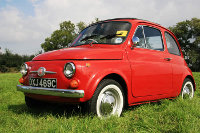
\includegraphics[width=0.5\textwidth]{output/car.jpg}}                
    \subfloat[First]{\label{fig:first1}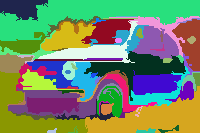
\includegraphics[width=0.5\textwidth]{output/op1.png}} \\               
    \subfloat[Second]{\label{fig:second1}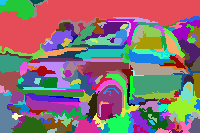
\includegraphics[width=0.5\textwidth]{output/tp1.png}}                
    \subfloat[Third, $R = 15$, $l = 8$]{\label{fig:third1}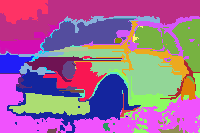
\includegraphics[width=0.5\textwidth]{output/r1-15-8.png}}                
\caption{RGB image 200x133 pixels, $K = 300$, $Min_c = 20$, $\sigma = 0.8$}
\label{fig:car200}
\end{figure}

\begin{figure}[htp]
    \centering
    \subfloat[Original]{\label{fig:original2}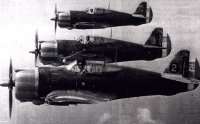
\includegraphics[width=0.5\textwidth]{output/planes-200.jpg}}                
    \subfloat[First, $K = 1000$, $Min_c = 15$, $\sigma = 0.5$]{\label{fig:first2}
\includegraphics[width=0.5\textwidth]{output/op5-1000-15.png}} \\               
    \subfloat[Second, $K = 300$, $Min_c = 15$, $\sigma = 0.8$]{\label{fig:second2}
\includegraphics[width=0.5\textwidth]{output/tp5-300-15.png}}                
    \subfloat[Third, $K = 300$, $Min_c = 15$, $\sigma = 0.8$, $R = 10$, $l = 7$]{\label{fig:third2}
\includegraphics[width=0.5\textwidth]{output/r5-10-7.png}}                
\caption{Greyscale image 200x124 pixels, Different parameters}
\label{fig:planes}
\end{figure}

\begin{figure}[htp]
    \centering
    \subfloat[Original]{\label{fig:original3}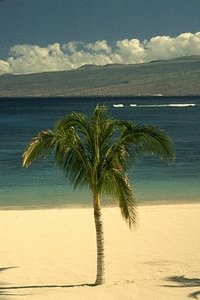
\includegraphics[width=0.5\textwidth]{output/beach.jpg}}                
    \subfloat[First]{\label{fig:first3}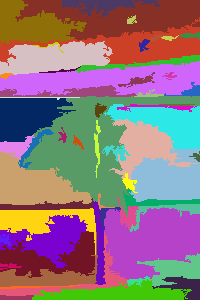
\includegraphics[width=0.5\textwidth]{output/op2-g05.png}} \\               
    \subfloat[Second]{\label{fig:second3}
\includegraphics[width=0.5\textwidth]{output/tp2-g05.png}}                
    \subfloat[Third, $R = 15$, $l = 8$]{\label{fig:third3}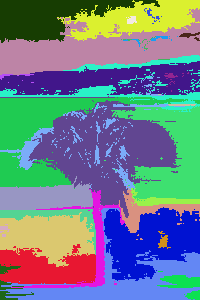
\includegraphics[width=0.5\textwidth]{output/r2-15-8-g05.png}}                
\caption{RGB image 200x300 pixels, $K = 500$, $Min_c = 50$, $\sigma = 0.5$}
\label{fig:beach}
\end{figure}
